\documentclass[10pt,a4paper]{article}
\setlength{\parindent}{0pt}
\addtolength{\oddsidemargin}{-.875in}
\addtolength{\evensidemargin}{-.875in}
\addtolength{\textwidth}{1.75in}
\addtolength{\topmargin}{-.875in}
\addtolength{\textheight}{1.75in}
\usepackage[utf8]{inputenc}
\usepackage{amsmath}
\usepackage{amsfonts}
\usepackage{amssymb}
\usepackage{setspace}
\usepackage{graphicx}
\onehalfspacing
\begin{document}
\begin{center}
{\Huge CS440 Homework 1}

Group Members: Nic Carchio, Zain Sayed, Ernest Lin
\end{center}
\part*{Questions}

\section*{Part 0 - Setup your Environments}
We generate our grid world environments by iterating through each cell in the 101 x 101 grid, assigning each one as blocked with 30\% probability, and the rest as unblocked. Then we randomly choose two pairs of coordinates to be the start and goal. We use pygame to visualize our mazes.
\section*{Part 1 - Understanding the methods}
\subsection*{a.}
In Figure 8, the agent is current at E2 and will explore the following cells (along with their g, h, and f values), with the "shortest presumed-unblocked path" assumption:
\newline\newline
E1: Unblocked, $g = 1, h = 4, f = 1 + 4 = 5$
\newline
D2: Unblocked, $g = 1, h = 4, f = 1 + 4 = 5$
\newline
E3: Unblocked, $g = 1, h = 2, f = 1 + 2 = 3$
\newline\newline
The move corresponding to the lowest $f$ value is E2 $\rightarrow$ E3, so the agent will travel to E3. Because the agent does not know initially which cells are blocked, it will travel to E3.
\subsection*{b.}
The agent 1) does not re-expand cells that are in the closed list (i.e. removed from the open list) and 2) will expand all cells that are in the same unblocked cell cluster (group of unblocked cells that can be reached between one another, or in other words, a connected graph of unblocked cells).
\newline\newline
There are a finite number of cells in the same unblocked cell cluster the agent can visit, so the agent will either 1) reach the target without expanding every cell or 2) expand every cell. In the first case, the agent just finds the path to the target. In the second case, if the target has not been found in the last possible cell the agent explored, then every cell is in the closed list and the agent discovers it's impossible to reach the target because no more moves can be done and no target has been found. If the target has been found, then the agent reaches the target. In all cases, because there is a finite number of unblocked cells the agent can expand and the agent doesn't re-expand cells in the closed list, it will either reach the target or discover that is impossible in finite time.
 \newline\newline
Below is the proof that the number of moves of the agent until it reaches the target or discovers that this is impossible is bounded from above by the number of unblocked cells squared:
 \newline\newline
 Let $m$ = number of moves of the agent (per computed normal A* path) until it reaches the target or discovers it's impossible, $u$ = number of unblocked cells in the grid world.
 \newline\newline
In each iteration of Repeated Forward A*, the path to the goal from the current cell is computed with normal A* and the "shortest presumed-unblocked path" assumption, and then the agent moves until it encounters a new blocked cell in its path, finds the target, or expanded all unblocked cells in its unblocked cell cluster. Between these 3 scenarios, the agent moves the most number of times if it encounters the last scenario, expanding all unblocked cells in its unblocked cell cluster, which can be at most $u$ if the agent can reach all unblocked cells in the gridworld. In other words,
\begin{center} $m \leq u$\end{center}

The agent wouldn't move more than the number of unblocked cells because the open list would be empty and the closed list would contain all unblocked cells it can reach. At this point, it would report that the target is found if the last cell is the target, otherwise it would report that the target cannot be found.

Again, in the worst case, the agent encounters a new blocked cell on its current path every time a new path is computed from normal A* in the Repeated Forward A* iteration. When this occurs, the agent must recompute a new A* path from its current cell, restarting its open list and closed list. However, the agent keeps new information on the blocked cells it discovers to ensure it won't get stuck on the same cell again, so the agent will recompute a new A* path AT MOST ONCE in each unblocked cell. If this is true, then the number of A* path computations, denoted by $c$, must be at most $u$, the number of unblocked cells in the gridworld, with the worst case including the scenario where the agent can reach all unblocked cells in the gridworld:
\begin{center} $c \leq u$\end{center}

Since $m$ is the number of agent moves for every normal A* path computation and $c$ is the number of normal A* computations, $mc$ is the total number of agent moves in the whole Repeated Forward A* algorithm. Using $m \leq u$ and $c \leq u$, it follows that the number of moves of the agent until it reaches the target or discovers that this is impossible is bounded above by the number of unblocked cells squared. In other words,
\begin{center} $mc \leq u^2$\end{center}

\section*{Part 2 - The Effects of Ties}
\subsection*{Figure 9 - Larger g-values in favor}
Step 0:\newline
OpenList: A1\newline
ClosedList: 
\newline\newline
Step 1:\newline
Remove A1 from OpenList\newline
A1's neighbors are A2, B1\newline
OpenList: A2($g = 1, h = 7, f = 8$), B1($g = 1, h = 7, f = 8$)\newline
ClosedList: A1
\newline\newline
Step 2:\newline
Remove A2 from OpenList (arbitrary)\newline
A2's neighbors are A1, B2, A3\newline
OpenList:  B2($g = 2, h = 6, f = 8$), A3($g = 2, h = 6, f = 8$), B1($g = 1, h = 7, f = 8$)\newline
ClosedList: A1, A2
\newline\newline
Step 3:\newline
Remove A3 from OpenList (largest $g$-value, arbitrary between A3 and B2)\newline
A3's neighbors are A2, A4, B3\newline
OpenList: A4($g = 3, h = 5, f = 8$), B3($g = 3, h = 5, f = 8$) B2($g = 2, h = 6, f = 8$), B1($g = 1, h = 7, f = 8$)\newline
ClosedList: A1, A2, A3
\newline\newline
Step 4:\newline
Remove A4 from OpenList (largest $g$-value, arbitrary between A4 and B3)\newline
A4's neighbors are A3, A5, B4\newline
OpenList: A5($g = 4, h = 4, f = 8$), B4($g = 4, h = 4, f = 8$), B3($g = 3, h = 5, f = 8$) B2($g = 2, h = 6, f = 8$), B1($g = 1, h = 7, f = 8$)\newline
ClosedList: A1, A2, A3, A4
\newline\newline
Step 5:\newline
Remove A5 from OpenList (largest $g$-value, arbitrary between A5 and B4)\newline
A5's neighbors are A4, B5\newline
OpenList: B5($g = 5, h = 3, f = 8$), B4($g = 4, h = 4, f = 8$), B3($g = 3, h = 5, f = 8$) B2($g = 2, h = 6, f = 8$), B1($g = 1, h = 7, f = 8$)\newline
ClosedList: A1, A2, A3, A4, A5
\newline\newline
Step 6:\newline
Remove B5 from OpenList (largest $g$-value)\newline
B5's neighbors are B4, C5
OpenList: C5($g = 6, h = 2, f = 8$), B4($g = 4, h = 4, f = 8$), B3($g = 3, h = 5, f = 8$) B2($g = 2, h = 6, f = 8$), B1($g = 1, h = 7, f = 8$)\newline
ClosedList: A1, A2, A3, A4, A5, B5
\newline\newline
Step 7:\newline
Remove C5 from OpenList (largest $g$-value)\newline
C5's neighbors are C4, D5
OpenList: C4($g = 7, h = 3, f = 10$), D5($g = 7, h = 1, f = 8$), B3($g = 3, h = 5, f = 8$) B2($g = 2, h = 6, f = 8$), B1($g = 1, h = 7, f = 8$)\newline
ClosedList: A1, A2, A3, A4, A5, B5, C5
\newline\newline
Step 8:\newline
Remove D5 from OpenList (largest $g$-value)\newline
D5's neighbors are D4, E5
OpenList: D4($g = 8, h = 2, f = 10$), E5($g = 8, h = 0, f = 8$) D5($g = 7, h = 1, f = 8$), B3($g = 3, h = 5, f = 8$) B2($g = 2, h = 6, f = 8$), B1($g = 1, h = 7, f = 8$)\newline
ClosedList: A1, A2, A3, A4, A5, B5, C5, D5
\newline\newline
Step 9:\newline
Remove E5 from OpenList (largest $g$-value)\newline
E5 is goal, so we stop.
\subsection*{Figure 9 - Smaller g-values in favor}
If cells with smaller $g$-values were prioritized, then the agent would expand all of the cells in a breadth-first-search manner, resulting in more cells expanded.
\subsection*{Implementation Conclusion}
To conclude, in general, Repeated Forward A* favoring larger g-values will be much faster than Repeated Forward A* favoring smaller g-values since the former will waste less time expanding cells closer to the start cell and will instead expand cells physically closer to the goal.
\subsection*{Implementation Comparison}
\begin{center}
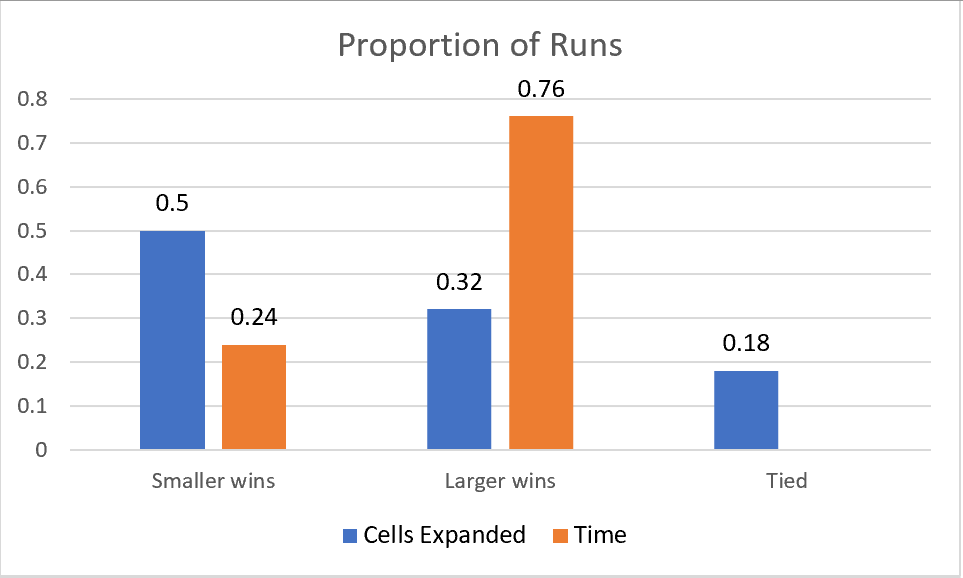
\includegraphics[scale = 1.0]{./graphs/part2_bar.png}
\newline
Figure 1: Repeated Forward A*, favoring larger g-values versus favoring smaller g-values, comparing Number of Cells Expanded and Run Time.
\newline
\end{center}
We ran Repeated Forward A* (RFA) on 50 different grid worlds. For each grid world, we ran RFA by breaking ties favoring smaller g-values and then by breaking ties favoring larger g-values.
\newline\newline
The blue columns in the bar graph in Figure 1 shos the proportion of the 50 runs where RFA favoring smaller g-values triumphed (fewer cells expanded) over RFA favoring larger g-values, vise versa, and the proportion where the two RFA versions tied. Thus, the bar graph indicates RFA favoring smaller g-values expands fewer cells than RFA favoring larger g-values 50\% (25 out of 50) of the runs, the opposite case happened in 32\% of the runs (16 out of 50), and tied in 18\% of the runs (9 out of 50).
\newline\newline
The orange columns show the proportion of the 50 runs where RFA favoring smaller g-values triumphed (less run time) over RFA favoring larger g-values and vise versa. RFA favoring larger g-values was faster than RFA favoring smaller g-values in 76\% of the runs (38 out of 50).
\newline\newline
Because of our analysis in Figure 9 of the assignment, we were initially surprised to see that RFA favoring larger g-values would expand more cells in more runs than RFA favoring smaller g-values. However, we noticed that the method of breaking of ties would primarily affect the number of cells expanded in the normal A* path computations within RFA, not necessarily the number of cells expanded by RFA itself. For every A* computation, RFA favoring smaller g-values expands many more cells than RFA favoring larger g-values, so the trend we see in run time being shorter with RFA favoring larger g-values than favoring smaller g-values makes sense. But after A* gives the current "shortest" path, RFA just follows that path, expanding every cell on the path until it hits the goal or another blocked cell, and this action is independent of the method of breaking ties and depends more on 1) the path returned by each version of RFA and 2) the grid world configuration. If, for some reason, A* favoring larger g-values returns paths that cause RFA's overall path (or equivalently, the number of expanded cells we're measuring) to be longer than those returned by A* favoring smaller g-values (which takes more run time per A* computation), then the results we see in our bar graph are very plausible. Therefore, our result show that although favoring larger g-values causes RFA to expand more cells overall, the run time is much shorter than favoring smaller g-values because A* path computations take longer with favoring smaller g-values.
\section*{Part 3 - Forward vs. Backward}
\begin{center}
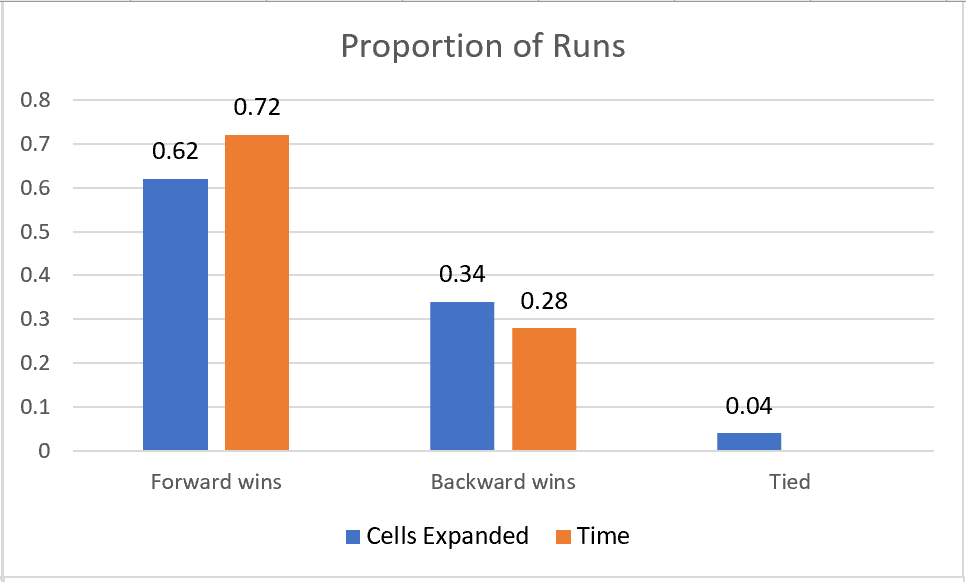
\includegraphics[scale = 1.0]{./graphs/part3_bar.png}
\newline
Figure 2: Repeated Forward A* versus Repeated Backward A*, comparing Number of Cells Expanded and Run Time and breaking ties favoring larger g-values.
\newline
\end{center}

In the 50 test runs, Repeated Forward A* (RFA) outperformed Repeated Backward A* (RBA) in terms of both the number of cells expanded and run time (RFA wins 62\% and 72\% of runs, respectively). This makes sense because every time A* computes a path on the known grid, most of the blocked cells are near the current cell. The current cell is the start node of A* in RFA, and because it is near most of the blocked cells, if A* encounters them in its path search, then it can easily expand other nodes that are close to the node it's currently on and maintains a relatively small open list. However, the current cell is the goal node of A* in RBA since it starts with the actual goal, so A* starts very far away from the blocked cells it knows, and when it hits a blocked cell, it expands other cells that are closest to the actual goal (RBA's start), causing the open list to not only be relatively larger but also have many cells with smaller f-values that are closer to the actual goal. Consider the 5 x 5 grid example below, which simulates the situation for RBA:
\newline\newline
\begin{center}
\begin{tabular}{ p{1.5cm}|p{1.5cm}|p{1.5cm}|p{1.5cm}|p{1.5cm}|p{1.5cm}| }
& 1 & 2 & 3 & 4 & 5\\[4ex]
 \hline
 A &  &  &  & BL & GOAL \\[4ex]
 \hline
 B &  &  &  & BL & \\[4ex]
 \hline
 C &  &  &  &  & \\[4ex]
 \hline
 D &  &  &  &  & \\[4ex]
 \hline
 E & START &  &  &  & \\[4ex]
 \hline
\end{tabular}
\newline
BL = blocked cell, START = starting cell of A*, GOAL = goal cell of A*
\end{center}
Assume the A* decides to move in the following shortest path, all the way to A3: E1 $\rightarrow$ D1 $\rightarrow$ C1 $\rightarrow$ B1 $\rightarrow$ A1 $\rightarrow$ A2 $\rightarrow$ A3. The f-values A* holds are the following:
\newline\newline
\begin{center}
\begin{tabular}{ p{1.5cm}|p{1.5cm}|p{1.5cm}|p{1.5cm}|p{1.5cm}|p{1.5cm}| }
& 1 & 2 & 3 & 4 & 5\\[4ex]
 \hline
 A & \textbf{f = 8} & \textbf{f = 8} & \textbf{f = 8} & BL & GOAL \\[4ex]
 \hline
 B & \textbf{f = 8} & f = 8\newline g = 4 & f = 10\newline g = 7 & BL & \\[4ex]
 \hline
 C & \textbf{f = 8} & f = 8\newline g = 3 &  &  & \\[4ex]
 \hline
 D & \textbf{f = 8} & f = 8\newline g = 2 &  &  & \\[4ex]
 \hline
 E & \textbf{START\newline f = 8} &  &  &  & \\[4ex]
 \hline
\end{tabular}
\newline
Bolded cell = Removed from open list and added to closed list (or equivalently, indicates the cell was expanded), Unbolded cell = In the open list (discovered but not expanded)
\end{center}
Because of the detour taken after A3, the f-value increased by at least 1 (by 2 in this case because B4 is blocked), so RBA decides to expand cells closer to the START than the GOAL since they have lower f-values.
\newline\newline
Under RFA, the START node and GOAL node are reversed but fewer cells would be expanded since the agent is immediately aware of the blocked cells at A4 and B4 after only 1 move. More specifically, the agent can only move A5 $\rightarrow$ B5 $\rightarrow$ C5, and after that it does not expand any useless cells since it dealt with the blocked areas much earlier and much closer to the start node at A5.
\newline\newline
For larger grids, such as our 101 x 101 grid worlds, RBA will expand many more useless cells than in the 5 x 5 grid, where the effect looks pretty minimal.
\newline\newline
Because blocked cells (in the known grid) are closer to the goal node in A* computations in RBA, RBA 1) expands more useless cells than RFA when detours occur and 2) holds more cells in its open list that are closer to its start node and have lower f-values from detours. Therefore, Repeated Forward A* performs better than Repeated Backward A* in most cases.
\section*{Part 4 - Heuristics in the Adaptive A*}
\subsection*{Proof 1}
\textbf{Prove that the Manhattan distances are consistent in gridworlds in which the agent can move only in the four main compass directions.}

The consistent property says:
\begin{center} $\forall(n, a, n'): h(n) \leq c(n, a, n') + h(n')$\end{center}

where $h(n)$ is the heuristic and $c(n, a, n')$ is the cost from node $n'$ to a successor of node $n$ by taking action $a$.

Assume the Manhattan distances are not consistent. That is,
\begin{center} $\exists(n, a, n'): h(n) > c(n, a, n') + h(n')$\end{center}

Rearranging,
\begin{center} $\exists(n, a, n'): h(n) - h(n') > c(n, a, n')$\end{center}

Case 1: If node $n'$ has a greater Manhattan distance to the goal node $G$ than node $n$, then $h(n')$ is greater than $h(n)$, which means $h(n) - h(n')$ is negative. Costs in the gridworld for moving from $n$ to $n'$ are always positive, so $h(n) - h(n') > c(n, a, n')$ cannot be true and is contradicted. Therefore, under case 1, the Manhattan distance is a consistent heuristic.
\newline\newline
Case 2: If node $n'$  has the same Manhattan distance to the goal node $G$ as node $n$, then $h(n')$ is the same as $h(n)$, which means $h(n) - h(n')$ is $0$. Costs in the gridworld for moving from $n$ to $n'$ are always positive, so $h(n) - h(n') > c(n, a, n')$ cannot be true and is contradicted. Therefore, under case 2, the Manhattan distance is a consistent heuristic.
\newline\newline
Case 3: If node $n'$ has a smaller Manhattan distance to the goal node $G$ than node $n$, then $h(n)$ is greater than $h(n')$, which means $h(n) - h(n')$ is positive. $h(n)$ and $h(n')$ are both Manhattan distances to the same goal node $G$, so $h(n) - h(n')$ is essentially the Manhattan distance between node $n$ and node $n'$, which we will denote with $h(n, n')$. Continuing from our earlier equation:
\begin{center} $\exists(n, a, n'): h(n, n') > c(n, a, n')$\end{center}

From the definition of Manhattan distance:
\begin{center} $\exists(n, a, n'): |x(n) - x(n')| + |y(n) - y(n')| > c(n, a, n')$\end{center}

We can think of $|x(n) - x(n')|$ and $|y(n) - y(n')|$ as the two legs of a triangle and $c(n, a, n')$ as the hypotenuse of the triangle. For such a $c(n, a, n')$ to exist so that the above inequality holds true, the agent must be allowed to move diagonally, which is not possible in our grid world. Because this isn't possible, the above inequality does not hold for any $(n, a, n')$. Therefore, by contradiction under case 3, the Manhattan distance is a consistent heuristic.

\subsection*{Proof 2}
\textbf{Prove that Adaptive A* leaves initially consistent h-values consistent even if action costs can increase.}

The Adaptive A* heuristic $hnew(s)$ is given by:
\begin{center} $hnew(s) = g(goal) - g(s) $\end{center}

where $g(goal)$ is the smallest cost to the goal node and $g(s)$ is the smallest cost to node $s$, both under current knowledge of the gridworld computed by the previous A* run, which expanded node $s$.

Plugging into the consistent property:
\begin{center} $\forall(n, a, n'): hnew(n) \leq c(n, a, n') + hnew(n')$\end{center}
\begin{center} $\forall(n, a, n'): g(goal) - g(n) \leq c(n, a, n') + g(goal) - g(n')$\end{center}
\begin{center} $\forall(n, a, n'): g(n') - g(n) \leq c(n, a, n')$\end{center}

Is there a case when $g(n') - g(n) > c(n, a, n')$? $c(n, a, n')$ is smallest when node $n$ is on a shortest path from node $s$ to node $n'$. In this scenario, $g(n') - g(n)$ is essentially the shortest distance between node $n$ and node $n'$, which is equivalent to or greater than $c(n, a, n')$ (equivalent if all cells between the two nodes are unblocked). Therefore, $g(n') - g(n) > c(n, a, n')$ cannot hold true for any $(n, a, n')$ which confirms that $\forall(n, a, n'): g(n') - g(n) \leq c(n, a, n')$ is true, so the Adaptive A* heuristic $hnew(s)$ is consistent even if action costs can increase.

\section*{Part 5 - Heuristics in the Adaptive A*}
\begin{center}
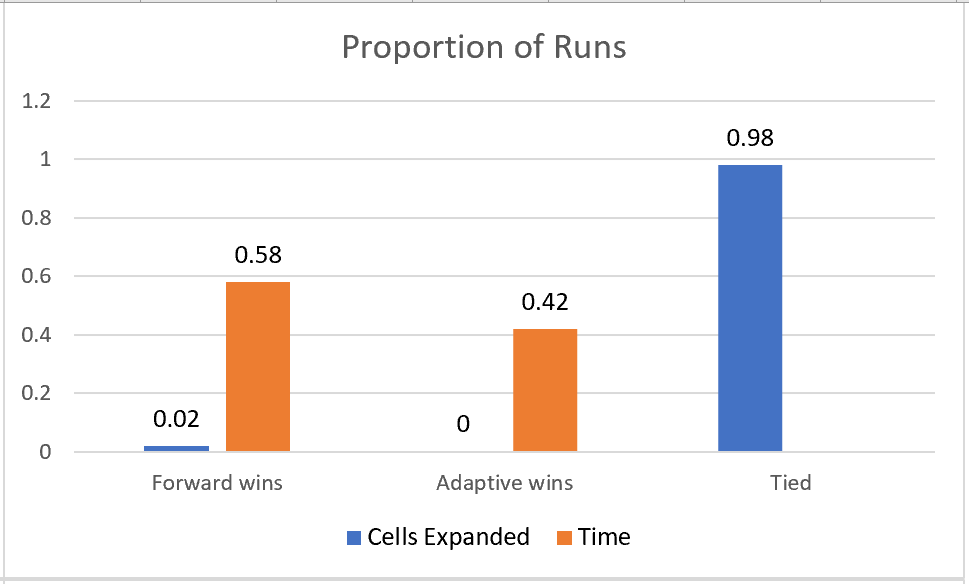
\includegraphics[scale = 1.0]{./graphs/part5_bar.png}
\newline
Figure 3: Repeated Forward A* versus Adaptive A*, comparing Number of Cells Expanded and Run Time, breaking ties with larger g-values.
\newline
\end{center}

In the 50 test runs, Repeated Forward A* (RFA) and Adaptive A* (AA) had about the same performance in terms of number of cells expanded (RFA wins 2\% of runs and the rest are ties), but RFA was slightly faster than AA in terms of run time (RFA wins 58\% of runs and AA wins 42\% of runs).

AA is supposed to be faster than RFA because it uses a larger heuristic that is still consistent, based on expanded cells in prior A* runs. In other words, AA supposedly makes more informed decisions on which node to remove from the open list than RFA in the A* path computations. The reason AA does not seem to add any improvement is most likely because when running A* in the known grid, all blocked cells are usually near the starting current cell, and the rest of the map (the majority) are presumed unblocked. The unblocked cells near the blocked cells at the start will be the only cells with their AA heuristic values updated somewhat significantly due to the blockage experience. Also, even if these presumed unblocked cells were expanded in prior A* computations, AA's heuristic for these cells was not much different than RFA's heuristic most of the time because the known grid was relatively more empty. Clearly from our results, the heuristic changes were insignificant since the number of cells expanded were equal between the two algorithms in 49 out of 50 runs, confirming our explanation above.
\newline\newline
We believe that our results show RFA performing slightly better than AA in terms of run time is because the cost of updating h-values outweighed the benefit of updating h-values. Searching through the closed list for every cell to try updating their h-values when computing A* paths is probably the main reason why AA took slightly longer in 58\% of the runs.
\section*{Part 6 - Memory Issues}
We only use two 2-D lists for the grids, which hold integers representing the color to display (indicating unblocked, blocked, start, goal, etc.), indexed by the x and y coordinates of the cell. One 2-D list stores the real grid, and the other 2-D list stores the grid with current information. In other words, each list entry stores only the integer color. We have 6 different values for color (only need 3 bits to represent), so we can reduce the memory by storing color in a 1-byte integer instead.

We have a separate class called "Treenode" that stores the $f$ (integer), $g$ (integer), $h$ (integer), Treenode parent (pointer), and coordinates 2-tuple (integer, integer). This adds up to 4 + 4 + 4 + 8 + 4 + 4 = 28 Bytes per Treenode. Depending on the grid size, the coordinates, $f$, $g$, and $h$ values can be compressed into smaller integers. For example, for the 101 x 101 grid, only 7 bits are required to represent an integer from 0 to 101. The x and y coordinates can be stored together in a 2-byte integer, with the x coordinate stored in the first 8 bits and the y coordinate stored in the last 8 bits (use bit shifts to access). As for the $h$ value in a 101 x 101 grid, the maximum value would be the largest Manhattan distance, 101 + 101 = 202, which can be represented by 1 Byte. The $f$ and $g$ values are upper bounded by 101 x 101 = 10201, so each can be represented by 14 bits, for a total of 28 bits, which can be accommodated by a 4-Byte integer. So the memory for one Treenode can be reduced from 28 Bytes to 4 ($f$ and $g$) + 1 ($h$) + 2 (x and y coordinates) + 8 (parent pointer) = 15 Bytes, assuming the compressions are possible.

For a gridworld of size 1001 x 1001, the memory to store our 2 grids would be:
\begin{center}
4 Bytes (color integer) * 101 * 101 * 2 (each grid) = 81608 Bytes
\end{center}

With a memory limit of 4 MBytes, the largest gridworld to operate on would be:
\begin{center}
4  * S * S * 2 = 4 * 1048576
\end{center}
\begin{center}
S = 724, or 724 x 724 gridworld.
\end{center}

The Treenodes are dynamically created and added to the open list as the A* algorithm runs, so we will exclude the memory used by Treenodes since that varies from grid to grid.

\end{document}

